\documentclass[../main.tex]{subfiles}

\begin{document}
	\section*{1 Лекция}
	\subsection*{Категорией С}
	\begin{enumerate}
		\item "Коллекция" объектов Obj(C)
		\item "Коллекция" морфизмов / стрелочек Mor(C) / Arr(C)
		\item \begin{mylist}
			\item $\forall x \in Obj(C) \exists f \in Arr(C): \begin{array}{l}
			f(X) = X\\
			f: X \rightarrow X\\
			(f, X) = X \text{ или }id_x
			\end{array}$
			\item $\forall f: X \rightarrow Y; g: Y \rightarrow Z$
			
			$f, g \in Arr(C)$\\
			$x, y, z \in Obj(C)$
			
			$\exists! h: X \rightarrow Z, h \in Arr(C)$
			
			$h = g \circ f$
			
			$\exists h!: X \rightarrow Z, h' \in Arr(C)$
			
			$h' = g \circ f$ -- запрещено
			\item
			
			$\forall a, b, c \in Arr(C)$
			
			$(a \circ b) \circ c = a \circ (b \circ c)$
		\end{mylist}
	\end{enumerate}
	
	$\forall f : X \rightarrow Y$
	
	$id_x: X \rightarrow X$
	
	$id_y: Y \rightarrow Y$
	
	$f \circ id_x = id_y \circ f = f$
	
	Примеры Категорий:
	\begin{mylist}
		\item Пустая категория
		\item $id_1$
		
		$id_1 \circ id_1 = id_1$
		\item \
		
		
\includegraphics[width=100px]{3кат}
		\item \
		
		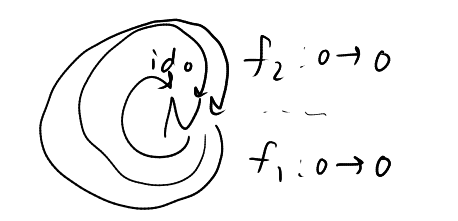
\includegraphics[width=150px]{4кат}
	\end{mylist}
	\begin{minipage}{\textwidth/2}
			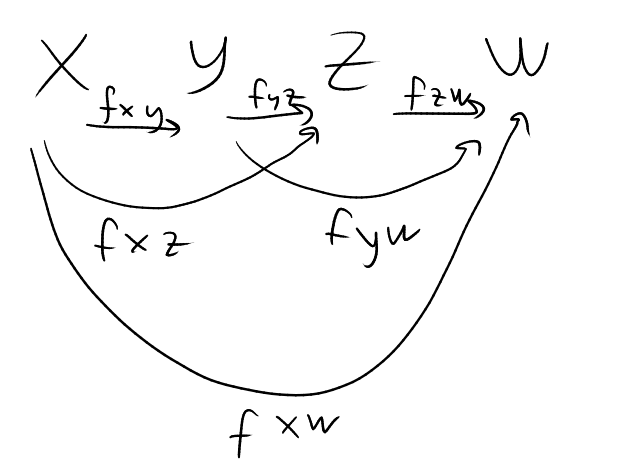
\includegraphics[width=\textwidth]{3}
	\end{minipage}
	\begin{minipage}{\textwidth/2}
		$f_{XW} = f_{ZW} \circ f_{XZ}$
		
		$f_{XW} = f_{YW} \circ f_{XY}$
		
		$f_{XW} = f_{ZW} \circ f_{YZ} \circ f_{XY}$
	\end{minipage}
	
	\begin{defin}
		Топосы -- множества + адекватное равенство + свободные структуры
	\end{defin}
	Свободные структуры -- всегда имеем понятие о том, как построен объект
	
\end{document}
